\documentclass{article}

\usepackage{iclr2026_conference,times}
%%%%% NEW MATH DEFINITIONS %%%%%

\usepackage{amsmath,amsfonts,bm}

% Mark sections of captions for referring to divisions of figures
\newcommand{\figleft}{{\em (Left)}}
\newcommand{\figcenter}{{\em (Center)}}
\newcommand{\figright}{{\em (Right)}}
\newcommand{\figtop}{{\em (Top)}}
\newcommand{\figbottom}{{\em (Bottom)}}
\newcommand{\captiona}{{\em (a)}}
\newcommand{\captionb}{{\em (b)}}
\newcommand{\captionc}{{\em (c)}}
\newcommand{\captiond}{{\em (d)}}

% Highlight a newly defined term
\newcommand{\newterm}[1]{{\bf #1}}


% Figure reference, lower-case.
\def\figref#1{figure~\ref{#1}}
% Figure reference, capital. For start of sentence
\def\Figref#1{Figure~\ref{#1}}
\def\twofigref#1#2{figures \ref{#1} and \ref{#2}}
\def\quadfigref#1#2#3#4{figures \ref{#1}, \ref{#2}, \ref{#3} and \ref{#4}}
% Section reference, lower-case.
\def\secref#1{section~\ref{#1}}
% Section reference, capital.
\def\Secref#1{Section~\ref{#1}}
% Reference to two sections.
\def\twosecrefs#1#2{sections \ref{#1} and \ref{#2}}
% Reference to three sections.
\def\secrefs#1#2#3{sections \ref{#1}, \ref{#2} and \ref{#3}}
% Reference to an equation, lower-case.
\def\eqref#1{equation~\ref{#1}}
% Reference to an equation, upper case
\def\Eqref#1{Equation~\ref{#1}}
% A raw reference to an equation---avoid using if possible
\def\plaineqref#1{\ref{#1}}
% Reference to a chapter, lower-case.
\def\chapref#1{chapter~\ref{#1}}
% Reference to an equation, upper case.
\def\Chapref#1{Chapter~\ref{#1}}
% Reference to a range of chapters
\def\rangechapref#1#2{chapters\ref{#1}--\ref{#2}}
% Reference to an algorithm, lower-case.
\def\algref#1{algorithm~\ref{#1}}
% Reference to an algorithm, upper case.
\def\Algref#1{Algorithm~\ref{#1}}
\def\twoalgref#1#2{algorithms \ref{#1} and \ref{#2}}
\def\Twoalgref#1#2{Algorithms \ref{#1} and \ref{#2}}
% Reference to a part, lower case
\def\partref#1{part~\ref{#1}}
% Reference to a part, upper case
\def\Partref#1{Part~\ref{#1}}
\def\twopartref#1#2{parts \ref{#1} and \ref{#2}}

\def\ceil#1{\lceil #1 \rceil}
\def\floor#1{\lfloor #1 \rfloor}
\def\1{\bm{1}}
\newcommand{\train}{\mathcal{D}}
\newcommand{\valid}{\mathcal{D_{\mathrm{valid}}}}
\newcommand{\test}{\mathcal{D_{\mathrm{test}}}}

\def\eps{{\epsilon}}


% Random variables
\def\reta{{\textnormal{$\eta$}}}
\def\ra{{\textnormal{a}}}
\def\rb{{\textnormal{b}}}
\def\rc{{\textnormal{c}}}
\def\rd{{\textnormal{d}}}
\def\re{{\textnormal{e}}}
\def\rf{{\textnormal{f}}}
\def\rg{{\textnormal{g}}}
\def\rh{{\textnormal{h}}}
\def\ri{{\textnormal{i}}}
\def\rj{{\textnormal{j}}}
\def\rk{{\textnormal{k}}}
\def\rl{{\textnormal{l}}}
% rm is already a command, just don't name any random variables m
\def\rn{{\textnormal{n}}}
\def\ro{{\textnormal{o}}}
\def\rp{{\textnormal{p}}}
\def\rq{{\textnormal{q}}}
\def\rr{{\textnormal{r}}}
\def\rs{{\textnormal{s}}}
\def\rt{{\textnormal{t}}}
\def\ru{{\textnormal{u}}}
\def\rv{{\textnormal{v}}}
\def\rw{{\textnormal{w}}}
\def\rx{{\textnormal{x}}}
\def\ry{{\textnormal{y}}}
\def\rz{{\textnormal{z}}}

% Random vectors
\def\rvepsilon{{\mathbf{\epsilon}}}
\def\rvtheta{{\mathbf{\theta}}}
\def\rva{{\mathbf{a}}}
\def\rvb{{\mathbf{b}}}
\def\rvc{{\mathbf{c}}}
\def\rvd{{\mathbf{d}}}
\def\rve{{\mathbf{e}}}
\def\rvf{{\mathbf{f}}}
\def\rvg{{\mathbf{g}}}
\def\rvh{{\mathbf{h}}}
\def\rvu{{\mathbf{i}}}
\def\rvj{{\mathbf{j}}}
\def\rvk{{\mathbf{k}}}
\def\rvl{{\mathbf{l}}}
\def\rvm{{\mathbf{m}}}
\def\rvn{{\mathbf{n}}}
\def\rvo{{\mathbf{o}}}
\def\rvp{{\mathbf{p}}}
\def\rvq{{\mathbf{q}}}
\def\rvr{{\mathbf{r}}}
\def\rvs{{\mathbf{s}}}
\def\rvt{{\mathbf{t}}}
\def\rvu{{\mathbf{u}}}
\def\rvv{{\mathbf{v}}}
\def\rvw{{\mathbf{w}}}
\def\rvx{{\mathbf{x}}}
\def\rvy{{\mathbf{y}}}
\def\rvz{{\mathbf{z}}}

% Elements of random vectors
\def\erva{{\textnormal{a}}}
\def\ervb{{\textnormal{b}}}
\def\ervc{{\textnormal{c}}}
\def\ervd{{\textnormal{d}}}
\def\erve{{\textnormal{e}}}
\def\ervf{{\textnormal{f}}}
\def\ervg{{\textnormal{g}}}
\def\ervh{{\textnormal{h}}}
\def\ervi{{\textnormal{i}}}
\def\ervj{{\textnormal{j}}}
\def\ervk{{\textnormal{k}}}
\def\ervl{{\textnormal{l}}}
\def\ervm{{\textnormal{m}}}
\def\ervn{{\textnormal{n}}}
\def\ervo{{\textnormal{o}}}
\def\ervp{{\textnormal{p}}}
\def\ervq{{\textnormal{q}}}
\def\ervr{{\textnormal{r}}}
\def\ervs{{\textnormal{s}}}
\def\ervt{{\textnormal{t}}}
\def\ervu{{\textnormal{u}}}
\def\ervv{{\textnormal{v}}}
\def\ervw{{\textnormal{w}}}
\def\ervx{{\textnormal{x}}}
\def\ervy{{\textnormal{y}}}
\def\ervz{{\textnormal{z}}}

% Random matrices
\def\rmA{{\mathbf{A}}}
\def\rmB{{\mathbf{B}}}
\def\rmC{{\mathbf{C}}}
\def\rmD{{\mathbf{D}}}
\def\rmE{{\mathbf{E}}}
\def\rmF{{\mathbf{F}}}
\def\rmG{{\mathbf{G}}}
\def\rmH{{\mathbf{H}}}
\def\rmI{{\mathbf{I}}}
\def\rmJ{{\mathbf{J}}}
\def\rmK{{\mathbf{K}}}
\def\rmL{{\mathbf{L}}}
\def\rmM{{\mathbf{M}}}
\def\rmN{{\mathbf{N}}}
\def\rmO{{\mathbf{O}}}
\def\rmP{{\mathbf{P}}}
\def\rmQ{{\mathbf{Q}}}
\def\rmR{{\mathbf{R}}}
\def\rmS{{\mathbf{S}}}
\def\rmT{{\mathbf{T}}}
\def\rmU{{\mathbf{U}}}
\def\rmV{{\mathbf{V}}}
\def\rmW{{\mathbf{W}}}
\def\rmX{{\mathbf{X}}}
\def\rmY{{\mathbf{Y}}}
\def\rmZ{{\mathbf{Z}}}

% Elements of random matrices
\def\ermA{{\textnormal{A}}}
\def\ermB{{\textnormal{B}}}
\def\ermC{{\textnormal{C}}}
\def\ermD{{\textnormal{D}}}
\def\ermE{{\textnormal{E}}}
\def\ermF{{\textnormal{F}}}
\def\ermG{{\textnormal{G}}}
\def\ermH{{\textnormal{H}}}
\def\ermI{{\textnormal{I}}}
\def\ermJ{{\textnormal{J}}}
\def\ermK{{\textnormal{K}}}
\def\ermL{{\textnormal{L}}}
\def\ermM{{\textnormal{M}}}
\def\ermN{{\textnormal{N}}}
\def\ermO{{\textnormal{O}}}
\def\ermP{{\textnormal{P}}}
\def\ermQ{{\textnormal{Q}}}
\def\ermR{{\textnormal{R}}}
\def\ermS{{\textnormal{S}}}
\def\ermT{{\textnormal{T}}}
\def\ermU{{\textnormal{U}}}
\def\ermV{{\textnormal{V}}}
\def\ermW{{\textnormal{W}}}
\def\ermX{{\textnormal{X}}}
\def\ermY{{\textnormal{Y}}}
\def\ermZ{{\textnormal{Z}}}

% Vectors
\def\vzero{{\bm{0}}}
\def\vone{{\bm{1}}}
\def\vmu{{\bm{\mu}}}
\def\vtheta{{\bm{\theta}}}
\def\va{{\bm{a}}}
\def\vb{{\bm{b}}}
\def\vc{{\bm{c}}}
\def\vd{{\bm{d}}}
\def\ve{{\bm{e}}}
\def\vf{{\bm{f}}}
\def\vg{{\bm{g}}}
\def\vh{{\bm{h}}}
\def\vi{{\bm{i}}}
\def\vj{{\bm{j}}}
\def\vk{{\bm{k}}}
\def\vl{{\bm{l}}}
\def\vm{{\bm{m}}}
\def\vn{{\bm{n}}}
\def\vo{{\bm{o}}}
\def\vp{{\bm{p}}}
\def\vq{{\bm{q}}}
\def\vr{{\bm{r}}}
\def\vs{{\bm{s}}}
\def\vt{{\bm{t}}}
\def\vu{{\bm{u}}}
\def\vv{{\bm{v}}}
\def\vw{{\bm{w}}}
\def\vx{{\bm{x}}}
\def\vy{{\bm{y}}}
\def\vz{{\bm{z}}}

% Elements of vectors
\def\evalpha{{\alpha}}
\def\evbeta{{\beta}}
\def\evepsilon{{\epsilon}}
\def\evlambda{{\lambda}}
\def\evomega{{\omega}}
\def\evmu{{\mu}}
\def\evpsi{{\psi}}
\def\evsigma{{\sigma}}
\def\evtheta{{\theta}}
\def\eva{{a}}
\def\evb{{b}}
\def\evc{{c}}
\def\evd{{d}}
\def\eve{{e}}
\def\evf{{f}}
\def\evg{{g}}
\def\evh{{h}}
\def\evi{{i}}
\def\evj{{j}}
\def\evk{{k}}
\def\evl{{l}}
\def\evm{{m}}
\def\evn{{n}}
\def\evo{{o}}
\def\evp{{p}}
\def\evq{{q}}
\def\evr{{r}}
\def\evs{{s}}
\def\evt{{t}}
\def\evu{{u}}
\def\evv{{v}}
\def\evw{{w}}
\def\evx{{x}}
\def\evy{{y}}
\def\evz{{z}}

% Matrix
\def\mA{{\bm{A}}}
\def\mB{{\bm{B}}}
\def\mC{{\bm{C}}}
\def\mD{{\bm{D}}}
\def\mE{{\bm{E}}}
\def\mF{{\bm{F}}}
\def\mG{{\bm{G}}}
\def\mH{{\bm{H}}}
\def\mI{{\bm{I}}}
\def\mJ{{\bm{J}}}
\def\mK{{\bm{K}}}
\def\mL{{\bm{L}}}
\def\mM{{\bm{M}}}
\def\mN{{\bm{N}}}
\def\mO{{\bm{O}}}
\def\mP{{\bm{P}}}
\def\mQ{{\bm{Q}}}
\def\mR{{\bm{R}}}
\def\mS{{\bm{S}}}
\def\mT{{\bm{T}}}
\def\mU{{\bm{U}}}
\def\mV{{\bm{V}}}
\def\mW{{\bm{W}}}
\def\mX{{\bm{X}}}
\def\mY{{\bm{Y}}}
\def\mZ{{\bm{Z}}}
\def\mBeta{{\bm{\beta}}}
\def\mPhi{{\bm{\Phi}}}
\def\mLambda{{\bm{\Lambda}}}
\def\mSigma{{\bm{\Sigma}}}

% Tensor
\DeclareMathAlphabet{\mathsfit}{\encodingdefault}{\sfdefault}{m}{sl}
\SetMathAlphabet{\mathsfit}{bold}{\encodingdefault}{\sfdefault}{bx}{n}
\newcommand{\tens}[1]{\bm{\mathsfit{#1}}}
\def\tA{{\tens{A}}}
\def\tB{{\tens{B}}}
\def\tC{{\tens{C}}}
\def\tD{{\tens{D}}}
\def\tE{{\tens{E}}}
\def\tF{{\tens{F}}}
\def\tG{{\tens{G}}}
\def\tH{{\tens{H}}}
\def\tI{{\tens{I}}}
\def\tJ{{\tens{J}}}
\def\tK{{\tens{K}}}
\def\tL{{\tens{L}}}
\def\tM{{\tens{M}}}
\def\tN{{\tens{N}}}
\def\tO{{\tens{O}}}
\def\tP{{\tens{P}}}
\def\tQ{{\tens{Q}}}
\def\tR{{\tens{R}}}
\def\tS{{\tens{S}}}
\def\tT{{\tens{T}}}
\def\tU{{\tens{U}}}
\def\tV{{\tens{V}}}
\def\tW{{\tens{W}}}
\def\tX{{\tens{X}}}
\def\tY{{\tens{Y}}}
\def\tZ{{\tens{Z}}}


% Graph
\def\gA{{\mathcal{A}}}
\def\gB{{\mathcal{B}}}
\def\gC{{\mathcal{C}}}
\def\gD{{\mathcal{D}}}
\def\gE{{\mathcal{E}}}
\def\gF{{\mathcal{F}}}
\def\gG{{\mathcal{G}}}
\def\gH{{\mathcal{H}}}
\def\gI{{\mathcal{I}}}
\def\gJ{{\mathcal{J}}}
\def\gK{{\mathcal{K}}}
\def\gL{{\mathcal{L}}}
\def\gM{{\mathcal{M}}}
\def\gN{{\mathcal{N}}}
\def\gO{{\mathcal{O}}}
\def\gP{{\mathcal{P}}}
\def\gQ{{\mathcal{Q}}}
\def\gR{{\mathcal{R}}}
\def\gS{{\mathcal{S}}}
\def\gT{{\mathcal{T}}}
\def\gU{{\mathcal{U}}}
\def\gV{{\mathcal{V}}}
\def\gW{{\mathcal{W}}}
\def\gX{{\mathcal{X}}}
\def\gY{{\mathcal{Y}}}
\def\gZ{{\mathcal{Z}}}

% Sets
\def\sA{{\mathbb{A}}}
\def\sB{{\mathbb{B}}}
\def\sC{{\mathbb{C}}}
\def\sD{{\mathbb{D}}}
% Don't use a set called E, because this would be the same as our symbol
% for expectation.
\def\sF{{\mathbb{F}}}
\def\sG{{\mathbb{G}}}
\def\sH{{\mathbb{H}}}
\def\sI{{\mathbb{I}}}
\def\sJ{{\mathbb{J}}}
\def\sK{{\mathbb{K}}}
\def\sL{{\mathbb{L}}}
\def\sM{{\mathbb{M}}}
\def\sN{{\mathbb{N}}}
\def\sO{{\mathbb{O}}}
\def\sP{{\mathbb{P}}}
\def\sQ{{\mathbb{Q}}}
\def\sR{{\mathbb{R}}}
\def\sS{{\mathbb{S}}}
\def\sT{{\mathbb{T}}}
\def\sU{{\mathbb{U}}}
\def\sV{{\mathbb{V}}}
\def\sW{{\mathbb{W}}}
\def\sX{{\mathbb{X}}}
\def\sY{{\mathbb{Y}}}
\def\sZ{{\mathbb{Z}}}

% Entries of a matrix
\def\emLambda{{\Lambda}}
\def\emA{{A}}
\def\emB{{B}}
\def\emC{{C}}
\def\emD{{D}}
\def\emE{{E}}
\def\emF{{F}}
\def\emG{{G}}
\def\emH{{H}}
\def\emI{{I}}
\def\emJ{{J}}
\def\emK{{K}}
\def\emL{{L}}
\def\emM{{M}}
\def\emN{{N}}
\def\emO{{O}}
\def\emP{{P}}
\def\emQ{{Q}}
\def\emR{{R}}
\def\emS{{S}}
\def\emT{{T}}
\def\emU{{U}}
\def\emV{{V}}
\def\emW{{W}}
\def\emX{{X}}
\def\emY{{Y}}
\def\emZ{{Z}}
\def\emSigma{{\Sigma}}

% entries of a tensor
% Same font as tensor, without \bm wrapper
\newcommand{\etens}[1]{\mathsfit{#1}}
\def\etLambda{{\etens{\Lambda}}}
\def\etA{{\etens{A}}}
\def\etB{{\etens{B}}}
\def\etC{{\etens{C}}}
\def\etD{{\etens{D}}}
\def\etE{{\etens{E}}}
\def\etF{{\etens{F}}}
\def\etG{{\etens{G}}}
\def\etH{{\etens{H}}}
\def\etI{{\etens{I}}}
\def\etJ{{\etens{J}}}
\def\etK{{\etens{K}}}
\def\etL{{\etens{L}}}
\def\etM{{\etens{M}}}
\def\etN{{\etens{N}}}
\def\etO{{\etens{O}}}
\def\etP{{\etens{P}}}
\def\etQ{{\etens{Q}}}
\def\etR{{\etens{R}}}
\def\etS{{\etens{S}}}
\def\etT{{\etens{T}}}
\def\etU{{\etens{U}}}
\def\etV{{\etens{V}}}
\def\etW{{\etens{W}}}
\def\etX{{\etens{X}}}
\def\etY{{\etens{Y}}}
\def\etZ{{\etens{Z}}}

% The true underlying data generating distribution
\newcommand{\pdata}{p_{\rm{data}}}
% The empirical distribution defined by the training set
\newcommand{\ptrain}{\hat{p}_{\rm{data}}}
\newcommand{\Ptrain}{\hat{P}_{\rm{data}}}
% The model distribution
\newcommand{\pmodel}{p_{\rm{model}}}
\newcommand{\Pmodel}{P_{\rm{model}}}
\newcommand{\ptildemodel}{\tilde{p}_{\rm{model}}}
% Stochastic autoencoder distributions
\newcommand{\pencode}{p_{\rm{encoder}}}
\newcommand{\pdecode}{p_{\rm{decoder}}}
\newcommand{\precons}{p_{\rm{reconstruct}}}

\newcommand{\laplace}{\mathrm{Laplace}} % Laplace distribution

\newcommand{\E}{\mathbb{E}}
\newcommand{\Ls}{\mathcal{L}}
\newcommand{\R}{\mathbb{R}}
\newcommand{\emp}{\tilde{p}}
\newcommand{\lr}{\alpha}
\newcommand{\reg}{\lambda}
\newcommand{\rect}{\mathrm{rectifier}}
\newcommand{\softmax}{\mathrm{softmax}}
\newcommand{\sigmoid}{\sigma}
\newcommand{\softplus}{\zeta}
\newcommand{\KL}{D_{\mathrm{KL}}}
\newcommand{\Var}{\mathrm{Var}}
\newcommand{\standarderror}{\mathrm{SE}}
\newcommand{\Cov}{\mathrm{Cov}}
% Wolfram Mathworld says $L^2$ is for function spaces and $\ell^2$ is for vectors
% But then they seem to use $L^2$ for vectors throughout the site, and so does
% wikipedia.
\newcommand{\normlzero}{L^0}
\newcommand{\normlone}{L^1}
\newcommand{\normltwo}{L^2}
\newcommand{\normlp}{L^p}
\newcommand{\normmax}{L^\infty}

\newcommand{\parents}{Pa} % See usage in notation.tex. Chosen to match Daphne's book.

\DeclareMathOperator*{\argmax}{arg\,max}
\DeclareMathOperator*{\argmin}{arg\,min}

\DeclareMathOperator{\sign}{sign}
\DeclareMathOperator{\Tr}{Tr}
\let\ab\allowbreak


\usepackage{amsmath}
\usepackage{amssymb}
\usepackage{booktabs}
\usepackage{graphicx}
\usepackage{microtype}
\usepackage{xcolor}
\usepackage{url}

\definecolor{draftblue}{RGB}{35,90,160}
\newcommand{\model}{\textsc{CGSM}}
\newcommand{\studentstate}{\texttt{<STUDENT\_STATE>}}
\newcommand{\draftnote}[1]{\textcolor{draftblue}{[\textbf{Draft:} #1]}}

\title{Beyond Correctness: Causally Grounded Generative Student Modeling\\
with Recurrent and Intervenable Student States}

\author{Anonymous authors}

% Uncomment only for a camera-ready version.
% \iclrfinalcopy

\begin{document}

\maketitle

\begin{abstract}
Student modeling is commonly divided into separate problems: predicting
correctness, forecasting a student's concrete response, diagnosing a
misconception, and estimating future behavior.  This fragmentation makes it
difficult to reuse evidence across tasks and limits most models to a fixed
label space or a task-specific prediction head.  We introduce \model, a
causally grounded generative student model that expresses these problems
through one conditional-generation interface and one recurrent student state.
After every observed interaction, a language-model updater compresses the
previous state and the new evidence into a continuous state carried by a
small bank of eight state slots addressed by one special token type.  A
task-conditioned decoder predicts correctness,
responses, misconceptions, prospective responses, or error recurrence from
this state and the query, without direct access to the history.  To make the
state predictive rather than merely decodable, we combine multi-task
generation with full-context distillation, recurrent--direct state
consistency, counterfactual supervision from executable misconceptions, and a
future-profile ownership objective.  We evaluate the model across six
educational data sources and separately test predictive sufficiency, temporal
updating, readable future profiles, state-ownership permutations, and
within-student stability.  The resulting framework turns student state from a
post-hoc activation into a compact computational object that can be cached,
updated, read, and audited.
\end{abstract}

\section{Introduction}
\label{sec:introduction}

What does a student know, and what will they do next?  Educational systems
usually operationalize this question as a collection of separate prediction
problems.  Knowledge tracing estimates whether the next response will be
correct \citep{corbett1995knowledge,piech2015deep,ghosh2020context}; cognitive
diagnosis associates performance with latent skills; response models predict
a selected option; and misconception systems explain a particular error.
These targets are related, but the models used to predict them rarely share an
interface.  A system that outputs a scalar probability of correctness cannot
directly say that a student is likely to add two denominators, produce the
resulting fraction, or preserve that error on a later problem without adding a
new task-specific output space.

This separation matters because correctness is a lossy description of student
behavior.  Two students can both answer incorrectly while producing different
responses for different reasons, and those differences determine which future
errors are plausible and which feedback would be appropriate.  Recent datasets
make richer modeling possible: Eedi links distractors to expert-authored
misconceptions \citep{wang2021diagnostic}; MalruleLib provides executable
mathematical error rules \citep{chen2026malrulelib}; and FoundationalASSIST
contains longitudinal problem text together with students' first responses
\citep{worden2026foundationalassist}.  Yet the dominant knowledge-tracing
formulation still maps an interaction sequence to a fixed correctness head.

Large language models (LLMs) offer a natural way to express heterogeneous
targets as conditional generation.  They can consume problem text, answer
choices, skill descriptions, and student histories in a shared context, then
emit either a class label or an open-form response.  However, using an LLM does
not by itself produce a valid student model.  A capable language model may
solve the problem rather than imitate the student, rely on item priors rather
than the student's history, or generate a plausible explanation unrelated to
the student's observed error.  Prior work has accordingly questioned whether
LLMs can simulate students under perturbed evidence \citep{sonkar2023deduction}
and whether apparent student simulations remain valid under stronger controls
\citep{yuan2026valid}.  A useful generative student model must therefore pass
both predictive and mechanistic tests: it should use student-specific evidence
to predict multiple outcomes, and its internal student representation should
have a demonstrable effect on those predictions.

We introduce \model, a causally grounded conditional-generation model with an
explicit recurrent student state.  After each observed interaction, a shared
language-model updater transforms the previous continuous state and the new
evidence into $z_t$.  A task-conditioned decoder then receives only $z_t$ and a
query; the raw history is unavailable as a bypass.  The same model produces
structured outputs for five constructs:
(i)~next-response correctness, (ii)~the student's concrete response,
(iii)~the misconception expressed by an observed error, (iv)~correctness and
response on a future problem after unobserved intervening interactions, and
(v)~the recurrence of the same wrong response on a later exposure.  The
formulation includes both closed-choice and open-generation protocols; it does
not average their unlike metrics into a single ``student modeling score.''

The main methodological challenge is to make $z_t$ sufficient for prediction
without sacrificing the performance of a full-context language model.  We use
four complementary objectives.  First, a full-context teacher distills its
output distribution into the state-only decoder.  Second, a trajectory
consistency loss aligns recurrently updated states with states independently
encoded from the corresponding complete history.  Third, executable
misconceptions provide counterfactual supervision: swapping a donor student's
state into a recipient query should generate the error obtained by applying the
donor's rule.  The last objective grounds state interventions behaviorally
rather than training an auxiliary misconception classifier.  Fourth, a
future-profile objective aligns a frozen view of the state with later
knowledge-component outcomes while teaching matched student--state ownership.

We evaluate the resulting state with a student-disjoint longitudinal protocol.
A readout selected only on training and validation students predicts held-out
future knowledge-component rates and emits readable weakness profiles.  We
compare it with a population prior and a same-window correctness/count
baseline, then permute state ownership across test students and compare two
disjoint views of each student's observed history.  The permutation asks
whether the right student's state matters; the disjoint-view test asks whether
the recovered information is stable.  Literal cross-student text transport is
reported as a diagnostic rather than a primary gate because an arbitrary
transplanted latent trajectory need not be in distribution.  This distinction
is essential because decodability alone does not establish a causal role
\citep{hewitt2019designing,elazar2021amnesic}.

We instantiate the framework with a 32B-parameter language model and a mixture
of six data sources spanning real longitudinal interaction logs, expert-labeled
misconceptions, and executable synthetic error rules.  Our formal evaluation
keeps students disjoint across longitudinal splits and separates temporal
prediction, non-temporal profile prediction, full-taxonomy misconception
retrieval, open generation, and controlled synthetic generalization.  This
protocol is deliberately stricter than evaluating against a row-specific set
of candidates known to contain the gold answer.  It also makes the limits of
each construct explicit: future performance within a knowledge component is
not treated as a direct mastery label, and repeated incorrectness without a
recorded response is not treated as persistence of the same misconception.

Our contributions are:
\begin{itemize}
    \item \textbf{A recurrent generative student state.} We cast correctness,
    concrete response prediction, misconception diagnosis, prospective
    behavior, and exact wrong-response recurrence as task-conditioned
    generation from one continuously updated state.
    \item \textbf{A construct-aware multi-source evaluation.} We align six
    educational data sources while preserving source-specific semantics and
    compare the unified model with classical and neural specialists, including
    IRT, PFA, BKT, DKT, AKT, retrieval, and response-frequency models.
    \item \textbf{Transfer across synthetic and authentic errors.} We test
    whether supervision from executable misconception rules improves diagnosis
    of expert-labeled errors, with task-matched ablations that distinguish rule
    supervision from merely adding synthetic responses.
    \item \textbf{Grounded state training.} Full-context distillation preserves
    predictive information, trajectory consistency teaches incremental
    updating, executable counterfactuals supervise task behavior, and future
    profile supervision binds states to student-specific outcomes.
    \item \textbf{A reusable, audited student state.} We combine held-out future
    prediction, readable profiles, state-ownership permutations, matched
    baselines, and disjoint-history stability to test whether the learned state
    is useful and student-specific.
\end{itemize}

Together, these contributions shift the question from whether a language model
can predict one educational label to whether one model can represent a
student's behavior at several levels of specificity---and whether the internal
state supporting those predictions can survive causal scrutiny.

\section{Related Work}
\label{sec:related-work}

\subsection{Knowledge tracing and student performance prediction}

Knowledge tracing (KT) estimates a student's evolving knowledge from a sequence
of learning interactions.  Bayesian Knowledge Tracing represents mastery of a
knowledge component with a hidden Markov model \citep{corbett1995knowledge},
while Performance Factors Analysis uses counts of prior successes and failures
as interpretable predictors \citep{pavlik2009performance}.  Item-response and
factor models instead explain outcomes through student ability and item
difficulty \citep{rasch1960probabilistic,vie2019knowledge}.  Neural KT replaces
hand-specified transitions with recurrent networks \citep{piech2015deep},
external memories \citep{zhang2017dynamic}, or self-attention
\citep{pandey2019self,ghosh2020context}.  These models are strong and appropriate
baselines for correctness prediction, but their standard objective and output
space remain task-specific: they estimate a binary outcome for an indexed item
or knowledge component.  Our work does not argue that such models are incapable
of richer prediction after modification.  Instead, we ask whether correctness,
concrete responses, misconception text, and prospective responses can be
handled by one generative interface without adding a separate prediction head
for every target.

The distinction also motivates our evaluation design.  Standard KT benchmarks
often emphasize warm-item, new-student prediction, where test students are held
out but most test items occurred during training.  Text-rich datasets such as
XES3G5M \citep{liu2023xes3g5m}, DBE-KT22
\citep{abdelrahman2022dbekt22}, and FoundationalASSIST
\citep{worden2026foundationalassist} permit models to use problem content in
addition to identifiers.  We retain student-disjoint temporal tests but report
protocols by data source and prediction type rather than pooling unlike label
spaces into a macro-average.

\subsection{Responses, misconceptions, and cognitive diagnosis}

Correctness does not identify the process that generated an answer.  Cognitive
diagnosis models infer mastery profiles over a predefined skill matrix
\citep{delatorre2009dina}, while distractor and misconception modeling links
particular wrong answers to systematic gaps in understanding.  The Diagnostic
Questions/Eedi benchmark made this connection explicit by associating
mathematics distractors with expert-authored misconceptions
\citep{wang2021diagnostic}.  More recently, MalruleLib formalized 101 executable
mathematical error rules and their step traces \citep{chen2026malrulelib}.  These
resources support complementary forms of evidence: Eedi provides authentic
expert labels for observed distractors, whereas MalruleLib provides controlled
counterfactual behavior and exact rule identity.

Our misconception task differs from ordinary per-example candidate ranking.
The main protocol either retrieves from the complete misconception taxonomy or
generates a diagnosis without exposing a candidate set constructed to contain
the gold label.  Our response tasks similarly distinguish closed-choice
prediction from open mathematical response generation.  This separation is
important: retrieving a supplied misconception and generating a student's
future response are not interchangeable capabilities, even when both can be
scored with semantic similarity.

\subsection{Language models as knowledge tracers and simulated students}

Recent work incorporates pretrained language models into KT to represent
question semantics and address cold-start items.  Language Model Can Do
Knowledge Tracing adapts language-model representations to KT
\citep{lee2024language}; CLST aligns a generative language model with a student
tracer for cold-start mitigation \citep{jung2024clst}; and SINKT combines
language-model semantics with structural information for inductive KT
\citep{fu2024sinkt}.  This line of work primarily retains correctness as the
prediction target.  It demonstrates the value of language semantics for KT but
does not by itself unify correctness with open responses and misconception
diagnosis.

A related line asks LLMs to act as students.  Sonkar and Baraniuk
\citeyearpar{sonkar2023deduction} probe whether LLMs follow provided student
evidence under perturbations.  Agent-based approaches condition LLMs on coarse
cognitive levels to generate imperfect behavior \citep{wu2025embracing}.
Contemporaneous work emphasizes that plausible generations are insufficient
evidence of valid student simulation and calls for comparisons against real
student behavior and stronger controls \citep{yuan2026valid}.  We share this
concern but study a different setting: the model is trained over actual student
histories and multiple predictive targets, rather than prompted to enact a
persona or ability level.  We also test whether history-dependent information
is localized in an internal state that can be intervened on.

\subsection{Probing and intervening on internal representations}

Linear probes are widely used to identify information encoded in neural
representations, but probe accuracy can reflect information that the model does
not use for its prediction.  Control tasks and selectivity analyses help
separate representation content from probe capacity \citep{hewitt2019designing},
while counterfactual removal or intervention tests whether an encoded feature is
behaviorally relevant \citep{elazar2021amnesic,ravfogel2021counterfactual}.
Accordingly, we do not treat a decodable student attribute as sufficient
evidence for a functional student state.

Our architecture goes beyond extracting a token activation from a complete
history.  It recurrently updates a compact continuous state and removes the raw
history from the prediction path.  Full-context distillation tests whether this
state preserves behaviorally useful information, while future-profile
supervision ties the state to later student outcomes.  At evaluation, a frozen
readout receives no history or student ID; permuting state ownership across
held-out students therefore tests whether the student-specific representation
matters.  Disjoint-history views test within-student stability, and population
and same-window outcome baselines test incremental utility.  We separately
report donor, same-profile, random, and no-op text-transport interventions as
diagnostics, without requiring arbitrary cross-student latent transplants to be
in distribution.

\section{Causally Grounded Generative Student Modeling}
\label{sec:method}

\subsection{Problem formulation}

Let $x_t=(q_t,r_t,y_t,k_t,m_t)$ denote an observed interaction at time $t$:
problem content $q_t$, student response $r_t$, correctness $y_t$, available
knowledge-component metadata $k_t$, and optional interaction metadata $m_t$.
Fields unavailable in a source are omitted rather than imputed.  The history
before a target is $H_t=(x_1,\ldots,x_{t-1})$.  Given a task instruction
$\tau$ and a target query $\tilde q_t$, we predict a structured textual output
$o_t$.

Standard generative prompting estimates
\begin{equation}
    p_\theta(o_t\mid \tau,H_t,\tilde q_t),
    \label{eq:full-context}
\end{equation}
which permits the decoder to retrieve arbitrary history tokens and does not
identify a student state.  We instead factor prediction through a fixed-size
continuous state:
\begin{align}
    z_t &= U_\theta(z_{t-1},x_{t-1}),
    \label{eq:update}\\
    p_\theta(o_t\mid \tau,z_t,\tilde q_t)
        &= G_\theta(\tau,z_t,\tilde q_t).
    \label{eq:decode}
\end{align}
The updater $U_\theta$ and decoder $G_\theta$ share the same language-model
backbone and parameter-efficient adapters.  The state
$z_t\in\mathbb{R}^{L\times S\times d}$ retains a layerwise trajectory with
$S=8$ slots, all addressed by one repeated \studentstate{} token type.  It is a
per-student, time-indexed activation, not a learned student-ID embedding.

The tasks differ only in when the state is read and which output fields are
requested.  T1 and T2 read the state before the target interaction; T3 first
updates the state with the observed wrong response and then requests a
misconception; T4 reads the current state but queries a problem $\Delta$
interactions in the future; and strict T5 updates with the current wrong
response before predicting its recurrence on a later exposure.  T6 predicts a
future-KC-performance band and is reported only as an appendix proxy, never as
a direct latent-mastery label.

\subsection{A recurrent state carried by eight slots}

We implement the updater with two banks of eight occurrences of the same
special token type.  For
an update, the model receives
\begin{equation}
 [\studentstate{}_{\mathrm{in}}^{1:S};\;\operatorname{serialize}(x_t);\;
  \studentstate{}_{\mathrm{out}}^{1:S}].
\end{equation}
All positions use the same tokenizer ID.  At the input positions, we replace
the ordinary token embeddings by projected and normalized copies of the
previous state,
\begin{equation}
    e_{\mathrm{in}}^{1:S}=P_{\mathrm{in}}\operatorname{LN}(z_t).
\end{equation}
The causal hidden activations at the output positions can attend to the
previous state and the new interaction; their layerwise trajectory becomes
\begin{equation}
    z_{t+1}=P_{\mathrm{out}}h(\studentstate{}_{\mathrm{out}}^{1:S}).
\end{equation}
For the first observed interaction, $z_0$ is initialized by a learned base
state associated with \studentstate{}.  The small projections $P_{\mathrm{in}}$ and
$P_{\mathrm{out}}$, layer-normalization parameters, and language-model adapters
are trained jointly.

At prediction time, the decoder receives
\begin{equation}
 [\operatorname{instruction}(\tau);\;\studentstate{}^{1:S};\;
  \operatorname{serialize}(\tilde q_t);\;o_t].
\end{equation}
The embeddings at \studentstate{} are replaced by
$P_{\mathrm{in}}\operatorname{LN}(z_t)$.  The raw history is not included, so
every history-dependent prediction must pass through the state.
This removes the history bypass that weakens one-shot bottleneck masks.  It also
makes inference incremental: a serving system stores one vector per student,
updates it after each interaction, and reuses it for any task query.

We unroll updates over chronological blocks and truncate gradients every $B$
interactions.  The state value is preserved across block boundaries while its
gradient is detached.  This bounds memory independently of the full student
history and permits training the 32B backbone with low-rank adapters.

\subsection{Multi-task structured generation}

All targets use a small structured output language.  Binary outcomes use
fields such as \texttt{<correctness>}; response tasks use
\texttt{<predicted\_response>}; misconception diagnosis uses
\texttt{<misconception>}; and prospective tasks combine multiple fields.  The
generative objective is the target-token negative log likelihood
\begin{equation}
    \mathcal L_{\mathrm{gen}}
    =-\sum_{j=1}^{|o_t|}\log
      p_\theta(o_{t,j}\mid o_{t,<j},\tau,z_t,\tilde q_t).
    \label{eq:gen-loss}
\end{equation}
Instruction, state, and query tokens are masked from the loss.  Task and source
samplers are separated so that a large correctness dataset does not dominate
open-response or misconception supervision.

This schema unifies the interface, not the construct or metric.  Closed-choice
responses remain distinct from open mathematical responses; Eedi diagnosis is
evaluated against its full taxonomy or by open generation; and strict
wrong-response recurrence is not merged with repeat-incorrectness proxies.

\subsection{Predictive state distillation}

A strict bottleneck can lose information before the updater learns useful
compression.  We therefore initialize a full-context teacher $T$ from the
strong unrestricted multi-task model.  For the same target, the teacher sees
$H_t$ as in Equation~\ref{eq:full-context}, while the student decoder sees only
$z_t$.  We minimize a temperature-scaled token-level divergence
\begin{equation}
    \mathcal L_{\mathrm{KD}}
    =\mathcal T^2\sum_j
      \operatorname{KL}\!\left(
      p_T^{(\mathcal T)}(\cdot\mid H_t,\tau,\tilde q_t,o_{t,<j})
      \;\|\;
      p_\theta^{(\mathcal T)}(\cdot\mid z_t,\tau,\tilde q_t,o_{t,<j})
      \right).
    \label{eq:kd-loss}
\end{equation}
The teacher is frozen.  Ground-truth generation remains the primary objective,
so the student is not forced to reproduce teacher errors.  The gap between the
teacher and state-only student is also reported as an empirical measure of
state sufficiency.

\subsection{Recurrent--direct state consistency}

Errors can accumulate when the state is updated over a long trajectory.  We
construct a second state from the complete visible history using a direct
history encoder $E_\theta$ with the existing late-fusion mask.  Its state token
can attend to all of $H_t$, but the answer cannot.  For selected checkpoints in
an unrolled trajectory, we align the recurrent state $z_t^{\mathrm{rec}}$ with
the stop-gradient direct state $z_t^{\mathrm{dir}}=E_\theta(H_t)$:
\begin{equation}
    \mathcal L_{\mathrm{dyn}}
      =1-\cos\!\left(
        \operatorname{LN}(z_t^{\mathrm{rec}}),
        \operatorname{sg}[\operatorname{LN}(z_t^{\mathrm{dir}})]
      \right).
    \label{eq:dyn-loss}
\end{equation}
We reverse the stop-gradient direction on half of the minibatches.  This
symmetric schedule prevents one branch from remaining an untrained target
while avoiding immediate representational collapse.  Both states must also
predict the same observed target through Equation~\ref{eq:gen-loss}; cosine
agreement alone is never optimized without behavioral supervision.

\subsection{Counterfactual grounding with executable misconceptions}

Decodability does not ensure that changing a state changes behavior.  We use
MalruleLib to construct supervised interventions.  Let histories $H^A$ and
$H^B$ instantiate different misconception rules $a$ and $b$, and let $q$ be a
held-out problem for which both rules are executable.  The library provides
counterfactual responses $r_a(q)$ and $r_b(q)$.  We decode the same query after
swapping the two states and optimize
\begin{align}
    \mathcal L_{\mathrm{cf}} ={}&
    -\log p_\theta(r_a(q)\mid z^A,\tau_{\mathrm{response}},q) \\
    &-\log p_\theta(r_b(q)\mid z^B,\tau_{\mathrm{response}},q).
    \label{eq:cf-loss}
\end{align}
The pairing procedure deliberately changes the problem template, so the model
cannot satisfy the loss by copying a previous answer.  We do not attach a
malrule classifier to $z$: the supervision specifies what the state should
\emph{do}, not which label a probe should recover.  Evaluation uses unseen
history--query pairs, held-out templates, and, where coverage permits, held-out
malrules.

\subsection{Future-profile ownership grounding}

To make student identity testable without exposing a student ID, we add an
auxiliary readout over a fixed projection $\phi(z_t)$ of the layerwise State8
trajectory.  For student $i$, let $y_i\in[0,1]^K$ be smoothed correctness rates
computed only from post-cutoff interactions and let $m_i$ mark KCs with
sufficient support.  A linear head predicts
\begin{equation}
    \hat y_i=\sigma(W\phi(z_i)+b).
\end{equation}
For a hard mismatched student $j$, selected inside the training split, we
optimize supported future-rate error together with an ownership margin:
\begin{align}
    \mathcal L_{\mathrm{prof}} &=
      \operatorname{MSE}_{m_i}(\hat y_i,y_i),\\
    \mathcal L_{\mathrm{own}} &=
      \max\{0,\gamma+
      \operatorname{MSE}_{m_i\cap m_j}(\hat y_i,y_i)-
      \operatorname{MSE}_{m_i\cap m_j}(\hat y_i,y_j)\}.
\end{align}
Post-cutoff targets supervise training but are never visible to the updater or
decoder at inference.  KCs below a threshold fixed from training support are
excluded from this auxiliary loss.

The complete objective is
\begin{equation}
    \mathcal L
      =\mathcal L_{\mathrm{gen}}
      +\lambda_{\mathrm{KD}}\mathcal L_{\mathrm{KD}}
      +\lambda_{\mathrm{dyn}}\mathcal L_{\mathrm{dyn}}
      +\lambda_{\mathrm{cf}}\mathcal L_{\mathrm{cf}}
      +\lambda_{\mathrm{prof}}\mathcal L_{\mathrm{prof}}
      +\lambda_{\mathrm{own}}\mathcal L_{\mathrm{own}}.
    \label{eq:total-loss}
\end{equation}
We first warm-start on unrestricted multi-task generation, then train recurrent
and direct state paths with distillation and consistency, and finally mix
counterfactual and profile batches with real-data replay.  This curriculum separates
language/output-format learning from state compression and reduces catastrophic
forgetting during causal grounding.

\section{Experiments}
\label{sec:experiments}

\draftnote{Populate from the formal evaluation manifest, not the obsolete
six-task matrix. Report every task by source and protocol.}

\subsection{Research Questions}

\begin{description}
    \item[RQ1: Generality.] Can one model remain competitive across correctness,
    response, misconception, and prospective-behavior tasks?
    \item[RQ2: Capability.] Can the model generate concrete responses, natural-
    language misconception diagnoses with evidence, prospective behavior, and
    persistence judgments that correctness-only KT does not natively expose?
    \item[RQ3: Transfer.] Does training on one educational task or supervision
    type improve a distinct held-out educational task under exposure-matched
    controls, including but not limited to synthetic-to-real diagnosis?
    \item[RQ4: State validity.] Does a frozen history-closed State8 predict and
    explain future behavior for unseen students, does pairing the state with
    its owner's outcomes matter, and are predictions stable across disjoint
    views of the same observed history?
\end{description}

\subsection{Datasets and Protocols}

\draftnote{Add the 259,845-example training table and 21,676-example formal
evaluation table, then separate T1, T2-choice, T2-open, T3-taxonomy,
T3-generation, T4 by prediction distance, and strict T5. Report T6
future-KC-performance only in the appendix.}

\subsection{Baselines and Metrics}

\draftnote{Describe IRT, PFA, BKT, DKT, AKT, conditional response models,
full-taxonomy retrieval, and persistence logistic regression. Do not compare
LLM-judge semantic accuracy and exact taxonomy accuracy as if identical.}

\subsection{Main Results}

\draftnote{Insert multi-seed results and confidence intervals. Current formal
matrix is suitable as a preliminary run, not a final ICLR table.}

\subsection{Method Ablations}

We compare: (i)~the unrestricted full-context model; (ii)~the existing
one-shot late-fusion bottleneck; (iii)~the recurrent architecture with only
$\mathcal L_{\mathrm{gen}}$; (iv)~variants removing distillation, trajectory
consistency, or counterfactual grounding; and (v)~the complete \model.  The
primary method diagnostic is the state-compression gap between the frozen
full-context teacher and the state-only decoder on identical examples.  We
also report accuracy or generation quality as a function of history length and
number of recurrent updates.

\subsection{Transfer and Student-State Analyses}

\draftnote{Add exposure-matched C3 ablations; State8 versus population and
same-window baselines; state-ownership permutation tests; disjoint-history
stability; readable future profiles; recurrent state drift; and one-shot
versus recurrent state comparisons.  Report literal donor, same-profile,
random, and no-op swaps as diagnostics rather than C4 gates.}

\subsection{Controlled Evidence for a One-Shot Causal State}
\label{sec:c4-one-shot}

We separately audit the strongest completed one-shot bottleneck, without
using it as evidence for recurrent closure.  On each frozen intervention pair,
the native recipient prediction is the recipient-rule response $B$.  We then
replace the residual stream at the single state-token address with either the
matched donor trajectory, norm-matched Gaussian residual noise, a same-rule
donor trajectory, or the recipient's own trajectory (no-op).  The primary
contrast is
\begin{equation}
    D_{\mathrm{specific}}
    = \Pr(\widehat r=r_A\mid\text{directed donor})
    - \Pr(\widehat r=r_A\mid\text{Gaussian noise}),
\end{equation}
computed only on pairs for which the native model predicts $B$.  Here
``random'' is deliberately an out-of-distribution Gaussian-noise control, not
a randomly selected student's state.

\begin{figure}[t]
    \centering
    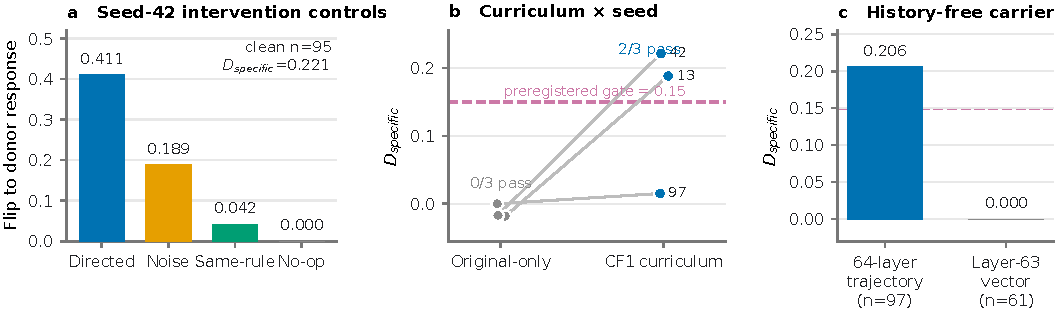
\includegraphics[width=\linewidth]{figures/c4_causal_state.pdf}
    \caption{\textbf{A causally specific one-shot student-state route is
    conditional on training and is carried across depth.}
    \captiona\ On the canonical CF1 + vision-pad seed-42 checkpoint, replacing
    the state-token trajectory with a matched donor trajectory changes the
    recipient prediction to the donor response in $0.411$ of the clean pairs,
    versus $0.189$ for norm-matched Gaussian noise, $0.042$ for a same-rule
    donor, and $0.000$ for no-op ($n=95$; $D_{\mathrm{specific}}=0.221$).
    \captionb\ The preregistered threshold $D_{\mathrm{specific}}\geq0.15$ is
    met by two of three historical CF1 runs but by none of the original-only
    runs; all seed-level results remain visible.  Thus the counterfactual
    curriculum is necessary in this factorial but is not sufficient across
    optimization runs.  The historical trainer did not seed model and LoRA
    construction before module initialization, so these are run-level rather
    than fully controlled training-seed replications.
    \captionc\ In a strict zero-training bridge, the decoder receives no raw
    history and has no persistent history KV cache.  Transferring the same
    address across all 64 residual layers preserves causal specificity
    ($D_{\mathrm{specific}}=0.206$, $n=97$), whereas transferring only its
    final layer-63 vector causes no prediction changes
    ($D_{\mathrm{specific}}=0$, $n=61$).  The completed evidence therefore
    supports a one-address, depth-indexed residual trajectory, not a compact
    final-layer vector or recurrent/Markov state.}
    \label{fig:c4-causal-state}
\end{figure}

\section{Conclusion}
\label{sec:conclusion}

\draftnote{Finalize after the full evaluation matrix and multi-seed C3/C4
experiments are complete.}

We presented a unified generative formulation for student modeling that moves
beyond correctness-only prediction toward concrete responses, misconceptions,
and prospective behavior.  The framework also exposes a designated internal
student state that can be evaluated with both probes and causal interventions.
For the primary state-validity claim, the intervention is a held-out
state-ownership permutation under a closed readout; literal cross-student text
transport remains diagnostic.
The current evidence supports the feasibility of this approach while
underscoring the importance of construct-aware evaluation: open generation is
not candidate retrieval, future performance is not a direct mastery label, and
decodability is not causality.


\bibliography{references}
\bibliographystyle{iclr2026_conference}

\appendix
\section{Task Prompts and Output Schemas}
\label{app:prompts}
\draftnote{Add one complete prompt and target example for each protocol.}

\section{Construct Validity and Data Audits}
\label{app:validity}
% Requires: \usepackage{booktabs}; \usepackage{graphicx}
% Counts are the post-filtering rows actually used by the unified training and
% formal-evaluation manifests (not the larger raw/source-level datasets).
\begin{table*}[t]
\centering
\caption{Datasets and task protocols in the unified student-modeling benchmark.
$N_{\mathrm{tr}}$, $N_{\mathrm{va}}$, and $N_{\mathrm{te}}$ are post-filtering
example counts.  Real educational logs and controlled synthetic data are
reported separately; a dash denotes that a source does not instantiate the
task.}
\label{tab:appendix_dataset_task_map}
\resizebox{\textwidth}{!}{%
\begin{tabular}{@{}lllp{4.0cm}rrrl@{}}
\toprule
Task & Source & Data type & Protocol / target & $N_{\mathrm{tr}}$ & $N_{\mathrm{va}}$ & $N_{\mathrm{te}}$ & Primary metric \\
\midrule
\textbf{T1: correctness}
 & DBE-KT22 & real, temporal & next-interaction first-response correctness; new-student/warm-item & 3,515 & 221 & 225 & Accuracy, AUROC \\
 & Eedi Response & real, non-temporal & held-out response conditioned on the same student's profile & 15,736 & 984 & 984 & Accuracy, AUROC \\
 & FoundationalASSIST & real, temporal & identifiable first-response correctness after support/privacy filtering & 30,009 & 1,863 & 1,882 & Accuracy, AUROC \\
 & XES3G5M & real, temporal & next-interaction correctness; official temporal test students & 52,009 & 2,888 & 7,222 & Accuracy, AUROC \\
 & MalRule & synthetic & systematic-rule correctness; same- and cross-template tests & 3,000 & 300 & 600 & Accuracy \\
\addlinespace
\textbf{T2: response}
 & DBE-KT22 & real, temporal & selected-option generation & 3,472 & 218 & 223 & Choice Acc. / MathEq \\
 & Eedi Response & real, non-temporal & profile-held-out option generation & 15,736 & 984 & 984 & Choice Acc. / MathEq \\
 & FoundationalASSIST & real, temporal & privacy-filtered structured mathematical first-response generation & 29,995 & 1,864 & 1,886 & MathEq \\
 & MalRule & synthetic & executable systematic-error response; same- and cross-template tests & 3,000 & 300 & 600 & MathEq \\
\addlinespace
\textbf{T3: diagnosis}
 & Eedi-Mining & real, response-level & open diagnosis against a 2,587-label expert misconception taxonomy; official fold 4 test & 3,476 & 0 & 894 & Semantic judge; retrieval MRR/$R@k$ \\
 & MalRule & synthetic & executable misconception identity; same- and cross-template tests & 3,000 & 300 & 600 & Label Acc.; semantic judge \\
\addlinespace
\textbf{T4: prospective behavior}
 & DBE-KT22 & real, temporal & correctness and selected response on a specified item at $\Delta=3$ & 3,186 & 200 & 200 & JointMath; CorrAcc \\
 & FoundationalASSIST & real, temporal & correctness and open response on a specified item at $\Delta\in\{1,3,5\}$ & 70,811 & 4,403 & 4,400 & JointMath; CorrAcc \\
\addlinespace
\textbf{T5: error persistence}
 & DBE-KT22 & real, temporal & same question and same wrong option recurs within the next three same-question records & 114 & 15 & 12 & AUROC, AUPRC, Acc. \\
 & FoundationalASSIST & real, temporal & exact normalized wrong first response recurs within the next three same-question records & 7,272 & 974 & 964 & AUROC, AUPRC, Acc. \\
\midrule
\multicolumn{4}{r}{\textbf{Total unique task examples}} & \textbf{244,331} & \textbf{15,514} & \textbf{21,676} & \\
\bottomrule
\end{tabular}%
}
\vspace{2pt}
\begin{minipage}{0.99\textwidth}\footnotesize
\textit{Protocol notes.} All real longitudinal splits are student-disjoint.
Eedi Response lacks timestamps in the public mirror and is therefore a
non-temporal profile-prediction protocol, not next-step KT. Eedi-Mining is a
response-level diagnosis set and contains no longitudinal student history.
MalRule is controlled synthetic evidence used for sanity checks,
cross-template generalization, transfer, and mechanism experiments; it is not
pooled with real data when making real-world performance claims. T6
(future-KC-performance band; legacy T4) is an appendix-only proxy and is not
included in the headline T1--T5 benchmark. Training counts use the original
training partition; the final one-epoch fit merged train and validation to
259,845 rows, while the frozen 21,676-row test set was never used for training.
\end{minipage}
\end{table*}

\begin{table}[t]
\centering
\caption{Appendix-only T6 future-KC-performance proxy.  The target is the
three-way band of correctness over up to five subsequent opportunities on the
same KC; it is not a direct latent-mastery label and is excluded from the
headline T1--T5 totals.}
\label{tab:appendix_t6_proxy}
\begin{tabular}{@{}lrrrl@{}}
\toprule
Source & $N_{\mathrm{tr}}$ & $N_{\mathrm{va}}$ & $N_{\mathrm{te}}$ & Primary metrics \\
\midrule
DBE-KT22 & 2,217 & 139 & 131 & Macro-F1, balanced Acc., QWK \\
XES3G5M & 20,561 & 1,131 & 2,808 & Macro-F1, balanced Acc., QWK \\
\midrule
Total & 22,778 & 1,270 & 2,939 & \\
\bottomrule
\end{tabular}
\end{table}

\begin{table*}[t]
\centering
\caption{Source-level scope and split construction. Question and student
counts describe the processed source before the final context-length filter.}
\label{tab:appendix_dataset_scope}
\resizebox{\textwidth}{!}{%
\begin{tabular}{@{}lp{3.0cm}rrlp{6.2cm}@{}}
\toprule
Source & Tasks used & Students & Questions / labels & History cap & Split and scope \\
\midrule
DBE-KT22 & T1, T2, T4, T5 & 1,193 & 212 questions & 6 & 954/119/120 train/validation/test students; temporal new-student, predominantly warm-item evaluation; multiple-choice database-education interactions. \\
Eedi Response & T1, T2 & 4,918 & 445 questions & 6 & 3,934/492/492 users; user-disjoint deterministic split. The mirror omits timestamps, so held-out examples measure profile-conditioned prediction rather than temporal forecasting. \\
FoundationalASSIST & T1, T2, T4, T5 & 5,000 & 2,986 questions & 12 & 4,000/500/500 students; temporal student-disjoint split. Free-text targets are conservatively filtered to privacy-safe structured mathematics; $\Delta=1,3,5$ for T4. \\
XES3G5M & T1 & 18,066 & 4,137 questions & 6 & 13,008/1,445/3,613 students; official temporal test users. The data record correctness but not the student's selected response, so they do not instantiate headline T2 or strict T5. \\
Eedi-Mining & T3 & -- & 2,587 labels & -- & 4,370 question--wrong-answer diagnosis queries; folds 0--3 (3,476) train and official fold 4 (894) test. No student sequence is present. \\
MalRule & T1, T2, T3 & synthetic & 21 rules; 132 surfaces & 4 & 3,000/300/600 synthetic profiles; the test combines 300 same-template and 300 cross-template profiles across fractions, decimals, and subtraction. \\
\bottomrule
\end{tabular}%
}
\end{table*}

\draftnote{Add the remaining construct-validity audit beyond the dataset and
task protocol tables.}

\end{document}
